%!TEX root = ../Demo.tex


\chapter{IoC 容器}
本章介绍了Spring的Inversion of Control(IoC)容器。

\section{Spring IoC容器和Beans简介}
本章介绍了 Spring 框架是如何实现控制反转(IoC)原则的。
IoC 又称为依赖注入(DI)。
通过依赖注入,对象与对象之间的依赖关系只
通过构造
函数参数、
工厂方法参数来声明,
还可以通过属性设置方法来声明这种依赖关系,
当对象被构造函数创建或者被工厂方法创建之后,可以通过属性设置方法来设置依赖关系。
当bean被创建时,容器会把这些依赖\textit{注入}进去。
因为这个过程叫控制反转,所以它是从根本上反转了以下过程:由bean自己通过构造函数实例化或查找依赖的对象和
由bean自己通过类似服务定位模式的设计模式来实例化或查找依赖对象

org.springframework.beans 和 org.springframework.context 
这两个包是Spring 框架的IoC 容器的基础包。BeanFactory接口实现了
一种可以管理任何类型的对象的高级配置机制。
ApplicationContext 是 BeanFactory 的一个子接口。
它可以更简单的与Spring的其他功能集成:

\begin{itemize}
    \item 与Spring的AOP特性轻松集成
    \item 消息资源处理(用于国际化)
    \item 事件发布
    \item 应用层面的上下文(如用于Web 应用的WebApplicationContext)
\end{itemize}

简而言之,BeanFactory提供了配置框架和基本功能,
ApplicationContext添加了更多企业定制的功能。
ApplicationContext是BeanFactory的完整超集,本章通过它来介绍Spring的IoC容器。
如果想了解更多关于BeanFactory的使用方法,可以参考\textbf{The BeanFactory}这一节。

在 Spring 中,Bean 是指那些构成系统应用的主要对象,它们由Spring的IoC容器初始化、组装和管理。
一个Bean 只是你应用中众多对象中的一个。
Bean 包括 Bean之间的依赖关系都通过\textit{配置元数据}来定义,
这些\textit{配置元数据}会被容器使用。

\section{容器概述}
org.springframework.context.ApplicationContext接口表示Spring IoC容器,
并负责实例化,配置和组装Bean。 
容器通过读取配置元数据来获取有关要实例化,配置和组装哪些对象的指令。 
配置元数据以XML,Java注解或Java代码表示。 
它使开发者能够表达组成应用程序的对象以及这些对象之间的丰富相互依赖关系。

Spring提供了ApplicationContext接口的几种实现。 
在独立应用程序中,通常创建ClassPathXmlApplicationContext
或FileSystemXmlApplicationContext的实例。 
尽管XML是定义配置元数据的传统格式,
但是可以通过提供少量XML配置来声明性地启用对这些其他元数据格式的支持
,例如Java注解或代码。

在大多数应用场景中,不需要显式的代码来实例化一个Spring IoC容器的一个或多个实例。 
例如,在Web应用程序场景中,应用程序的web.xml文件中简单的八行(约)
模板Web描述符XML通常就足够了(请参阅Web应用程序的便捷ApplicationContext实例化)。
 如果使用Spring Tools for Eclipse(Eclipse支持的开发环境),
 则只需单击几下鼠标或击键即可轻松创建此样板配置。

 下图描绘了Spring的大致工作原理。 
 应用程序类与配置元数据会被结合在一起,
 在创建和初始化ApplicationContext之后,会产出一个完全配置且可执行的系统或应用程序。

 \begin{figure}[ht]
    \centering
    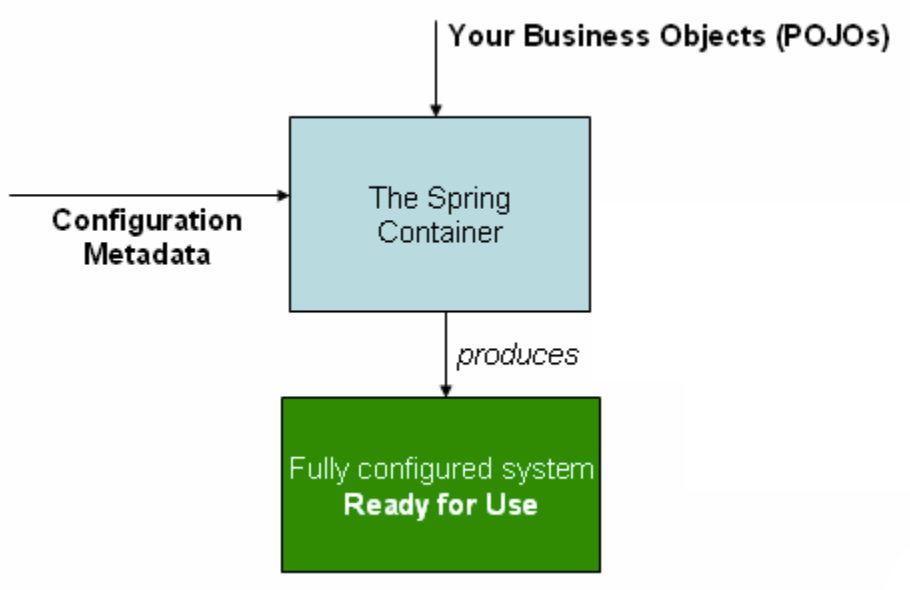
\includegraphics[width=0.6\linewidth]{./Figure/IMG_process.png}
    \caption{Spring IoC 容器}\label{Fig:xd1}
  \end{figure}

\subsection{配置元数据}
如上图所示,Spring IoC容器使用某种形式的配置元数据。 
此配置元数据表示应用程序开发人员如何告诉Spring容器实例化,配置和组装应用程序中的对象。

大多情况下,配置元数据以简单直观的XML格式提供,
因此本章大部分内容用XML格式的配置元数据来介绍Spring IoC容器的关键概念和功能。

有关在Spring容器中其他形式的元数据的使用,请参见:

\begin{itemize}
    \item 基于注解的配置:Spring 2.5引入了对基于注解的配置元数据的支持。
    \item 基于Java的配置:从Spring 3.0开始,
    Spring JavaConfig项目提供的许多功能成为核心Spring Framework的一部分。 
    因此,可以使用Java而不是XML文件来定义应用程序类外部的bean。
     要使用这些新功能,请参见@ Configuration,@ Bean,@ Import和@DependsOn注解。
\end{itemize}

Spring配置由至少一个(通常是一个以上)容器管理的bean定义组成。 
基于XML的配置元数据将这些bean配置为顶级<beans/>元素内的<bean/>元素。
Java配置通常在@Configuration类中使用@Bean注释的方法。

这些bean定义对应于组成应用程序的实际对象。
通常,开发者定义服务层对象、数据访问对象(DAO)、表示对象(例如Struts Action实例)、基础结构对象(例如Hibernate SessionFactories,JMS队列)等等。
通常,开发者不会在容器中配置细粒度的域对象,因为DAO和业务逻辑通常负责它们的创建和加载。
但是,可以使用Spring与AspectJ的集成来配置在IoC容器的控制范围之外创建的对象。
请参阅使用AspectJ与Spring依赖注入域对象。

\newpage
以下示例显示了基于XML的配置元数据的基本结构:

\begin{figure}[ht]
    \centering
    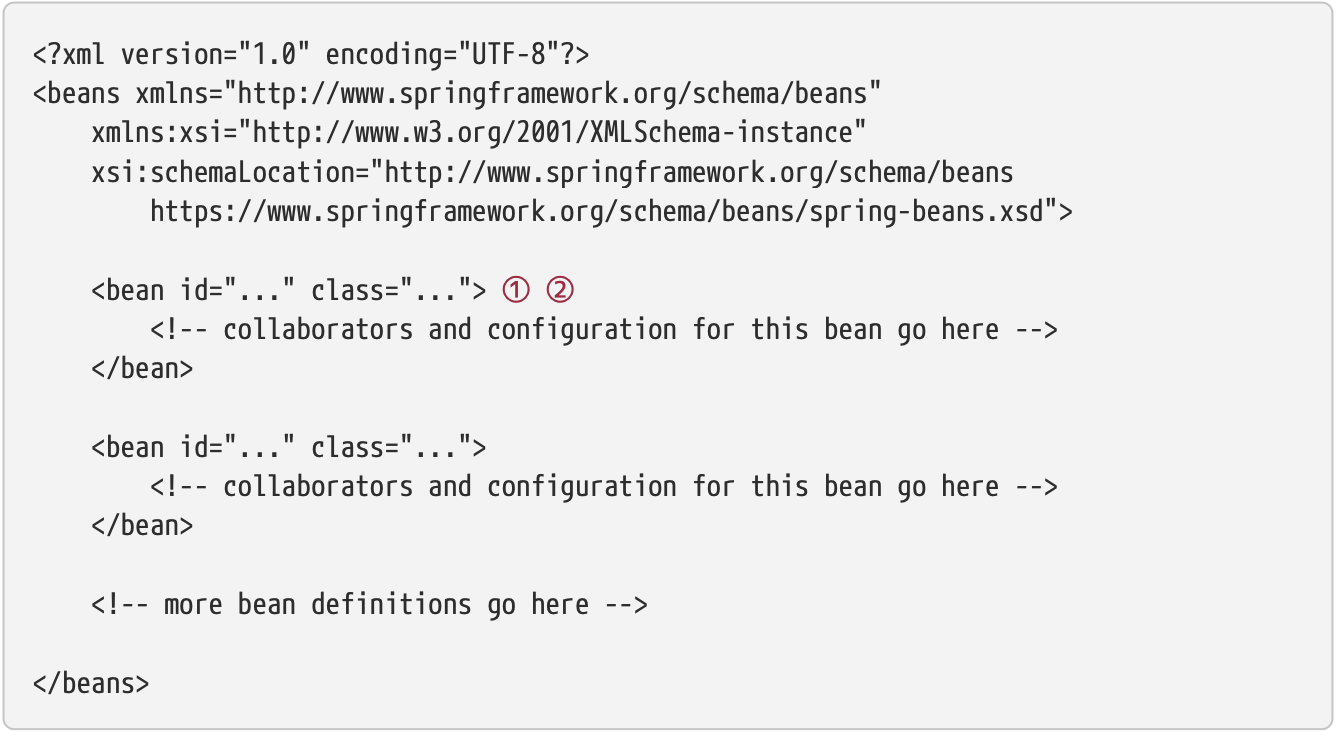
\includegraphics[width=1\linewidth]{./Figure/IMG_code_1.png}
  \end{figure}

\begin{enumerate}
    \item id属性是一个标识单个bean定义的字符串。
    \item class属性定义bean的类型,并使用完全限定的类名。
\end{enumerate}

id属性的值可以作为对象引用,并在其他bean 定义中被引用。 
在此示例中未描述如何进行对象引用。 有关更多信息,请参见依赖项。

\subsection{实例化容器}
ApplicationContext构造函数的参数是表示资源位置路径的字符串,
这些资源字符串使容器可以从各种外部资源(例如本地文件系统,Java CLASSPATH等)加载配置元数据。

\begin{figure}[ht]
\centering
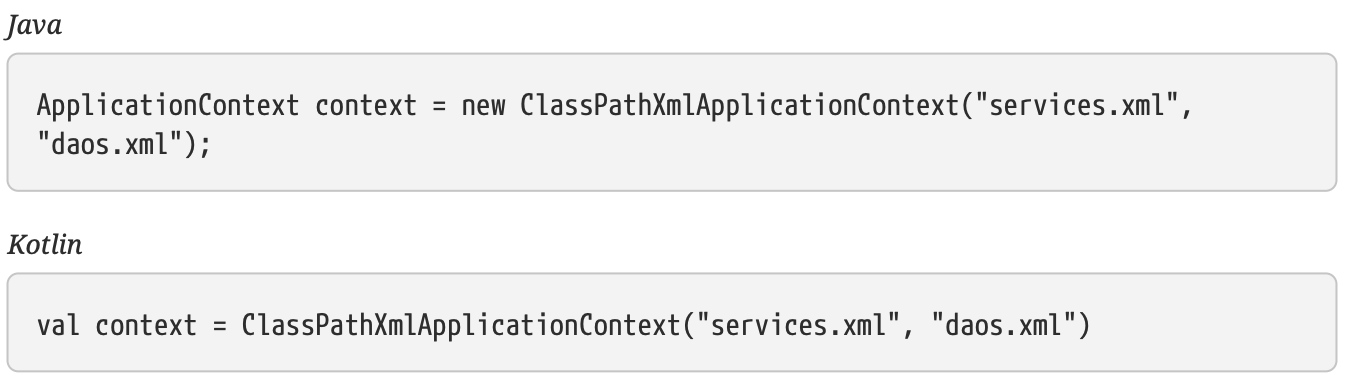
\includegraphics[width=1\linewidth]{./Figure/IMG_code_2.png}
\end{figure}

\newpage
以下示例显示了服务层对象(services.xml)的配置文件:

\begin{figure}[ht]
\centering
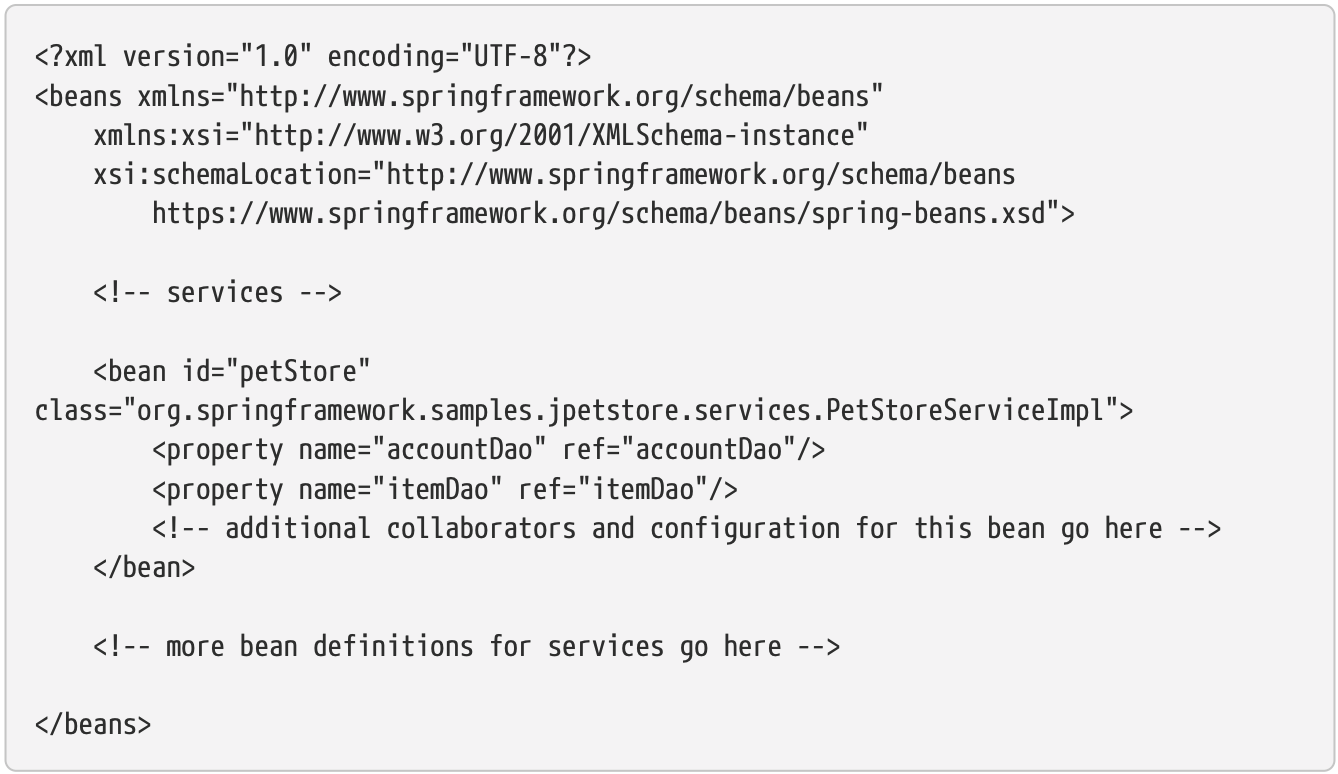
\includegraphics[width=1\linewidth]{./Figure/IMG_code_3.png}
\end{figure}

以下示例显示了数据访问对象(daos.xml)文件:

\begin{figure}[ht]
\centering
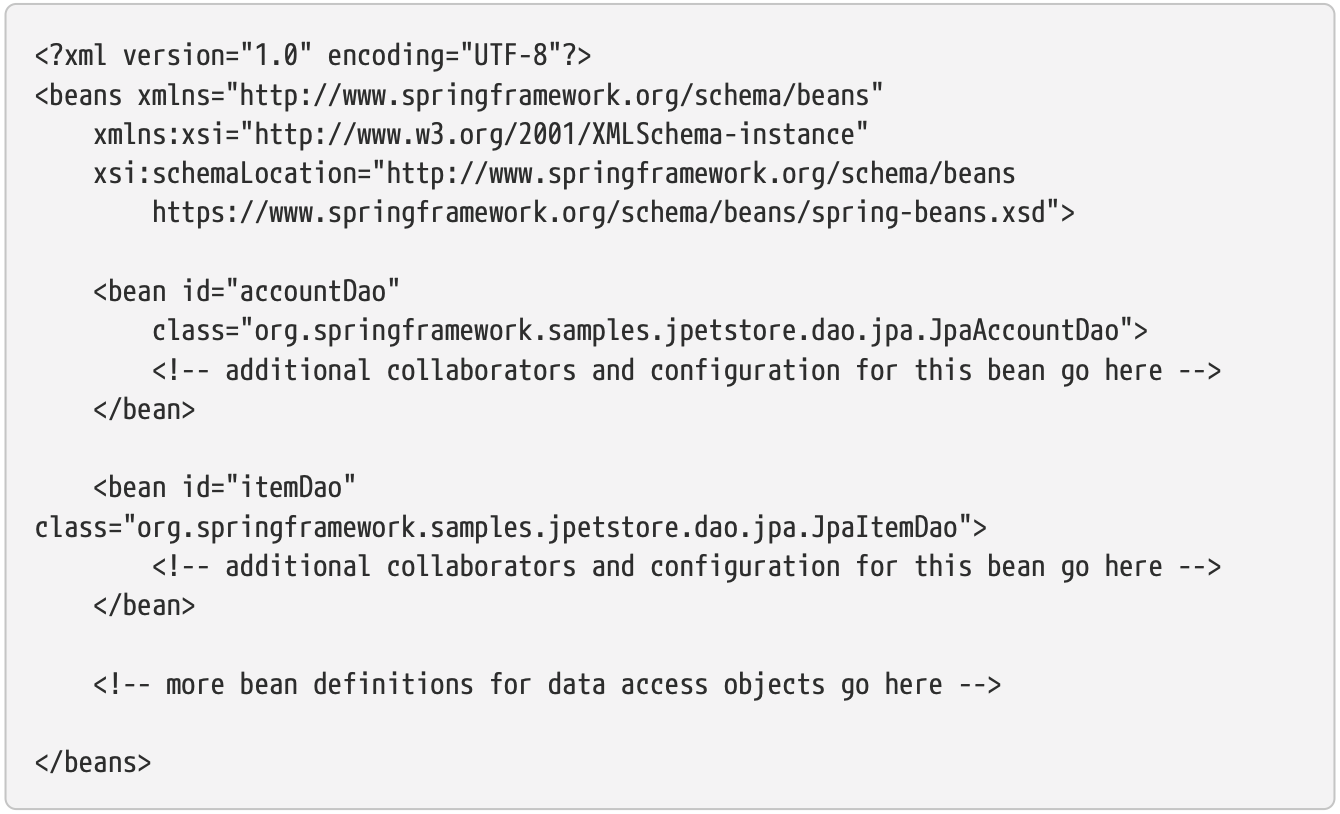
\includegraphics[width=1\linewidth]{./Figure/IMG_code_4.png}
\end{figure}

在前面的示例中,服务层由PetStoreServiceImpl类和两个JpaAccountDao
和JpaItemDao类型的数据访问对象组成(基于JPA对象关系映射标准)。
 属性名称元素引用JavaBean属性的名称,而ref元素引用另一个bean定义的名称。 
 id和ref元素之间的这种联系表达了协作对象之间的依赖性。 
 有关配置对象的依存关系的详细信息,请参阅依存关系。

 \subsubsection{组合基于XML的配置元数据}
 使bean定义跨越多个XML文件可能会很有用。 
 通常,每个单独的XML配置文件都代表体系结构中的逻辑层或模块。

 您可以使用应用程序上下文构造函数从所有这些XML片段中加载bean定义。 
 如上一节中所示,此构造函数具有多个Resource位置。
  或者,使用一个或多个出现的<import/>元素从另一个文件中加载bean定义。 
  以下示例显示了如何执行此操作:

  \begin{figure}[ht]
    \centering
    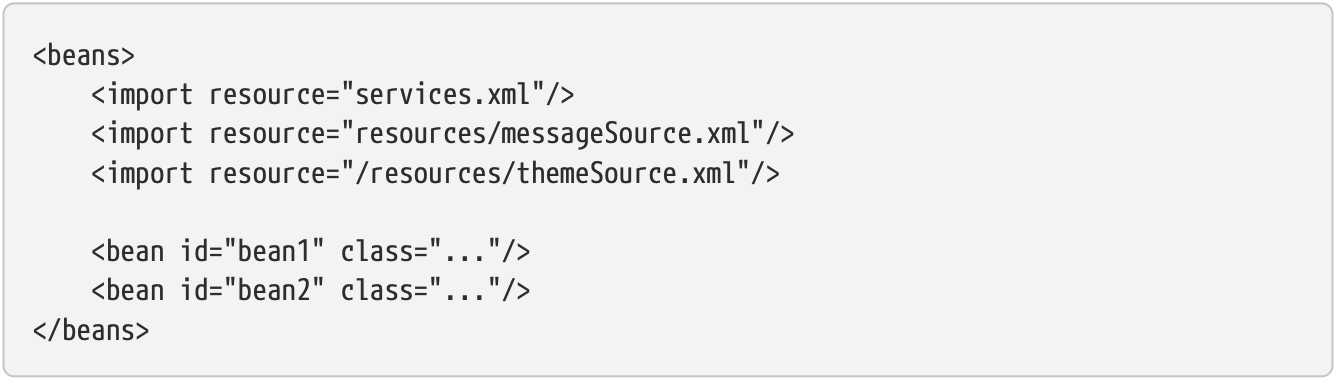
\includegraphics[width=1\linewidth]{./Figure/IMG_code_5.png}
    \end{figure}

    在前面的示例中,外部bean定义是从以下三个文件加载的:services.xml,messageSource.xml和themeSource.xml。 
    所有位置路径都相对于进行导入的定义文件,因此,services.xml必须与进行导入的文件位于同一目录或类路径位置,
    而messageSource.xml和themeSource.xml必须位于进行导入的文件的位置下方的资源位置。 
    如您所见,斜杠被忽略。 但是,鉴于这些路径是相对的,最好不要使用任何斜线。 
    根据Spring Schema,导入的文件的内容(包括顶级<beans />元素)必须是有效的XML bean定义。

    命名空间本身提供了导入指令功能。 
    Spring中的一系列XML名称空间(例如,上下文和util名称空间)
    提供了超出普通bean定义的其他配置功能。

\subsubsection{Groovy Bean定义DSL}
作为外部化配置元数据的另一个示例,
Bean定义也可以在Spring的Groovy Bean定义DSL中表达,
类似Grails。 
通常,这种配置位于“.groovy”文件中,其结构如以下示例所示:

\begin{figure}[ht]
    \centering
    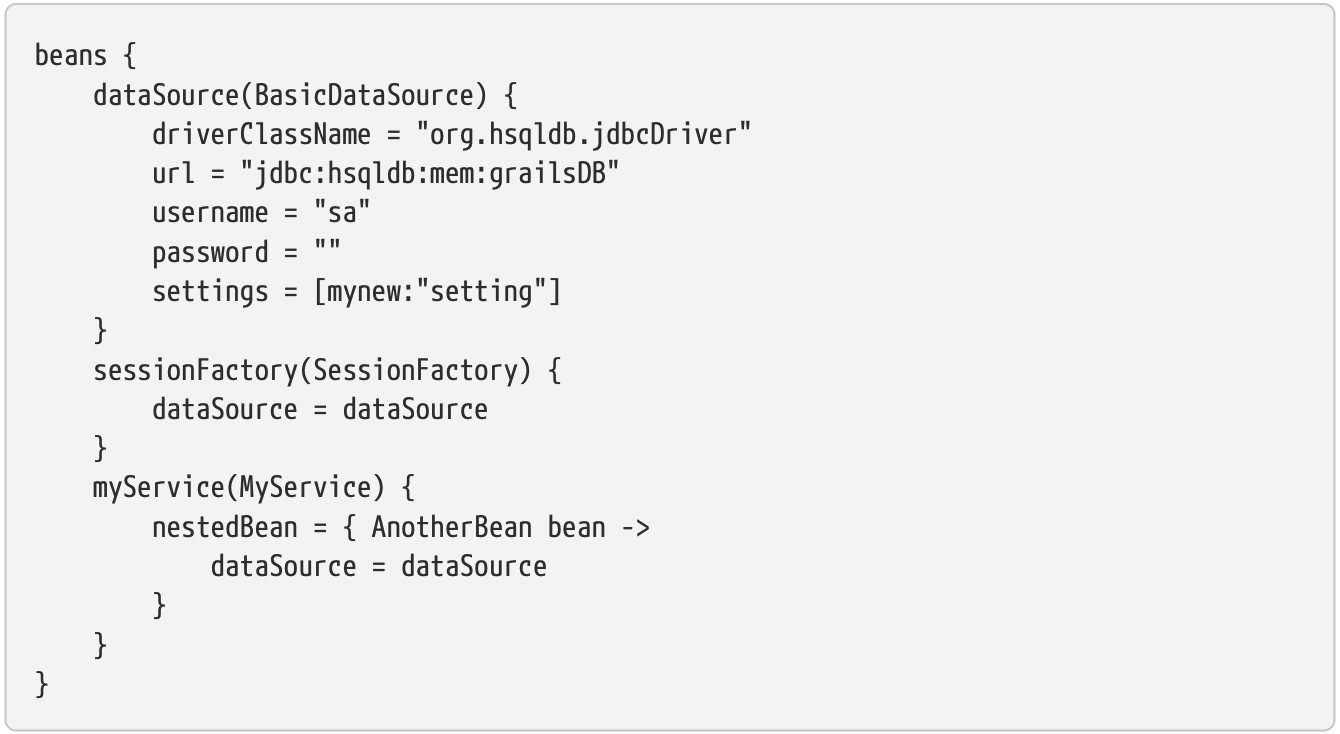
\includegraphics[width=1\linewidth]{./Figure/IMG_code_6.png}
    \end{figure}
    

\section{Bean概述}
Spring IoC容器管理一个或多个bean。 
这些bean是使用开发者提供给容器的配置元数据创建的(例如,以XML <bean/>定义的形式)。 
在容器本身内,这些bean定义表示为BeanDefinition对象,其中包含(除其他信息外)以下元数据:

\begin{itemize}
    \item 包限定的类名:定义了Bean的实际实现类。
    \item Bean行为配置元素,用于声明Bean在容器中的行为(作用域,生命周期回调等)。
    \item 引用其他bean来完成其工作所需要的。 这些引用也称为协作者或依赖项。
    \item 要在新创建的对象中设置的其他配置设置-例如,池的大小限制或要在管理连接池的bean中使用的连接数。
\end{itemize}

% 此元数据转换为构成每个bean定义的一组属性。 下表描述了这些属性:

% \begin{figure}[ht]
%     \centering
%     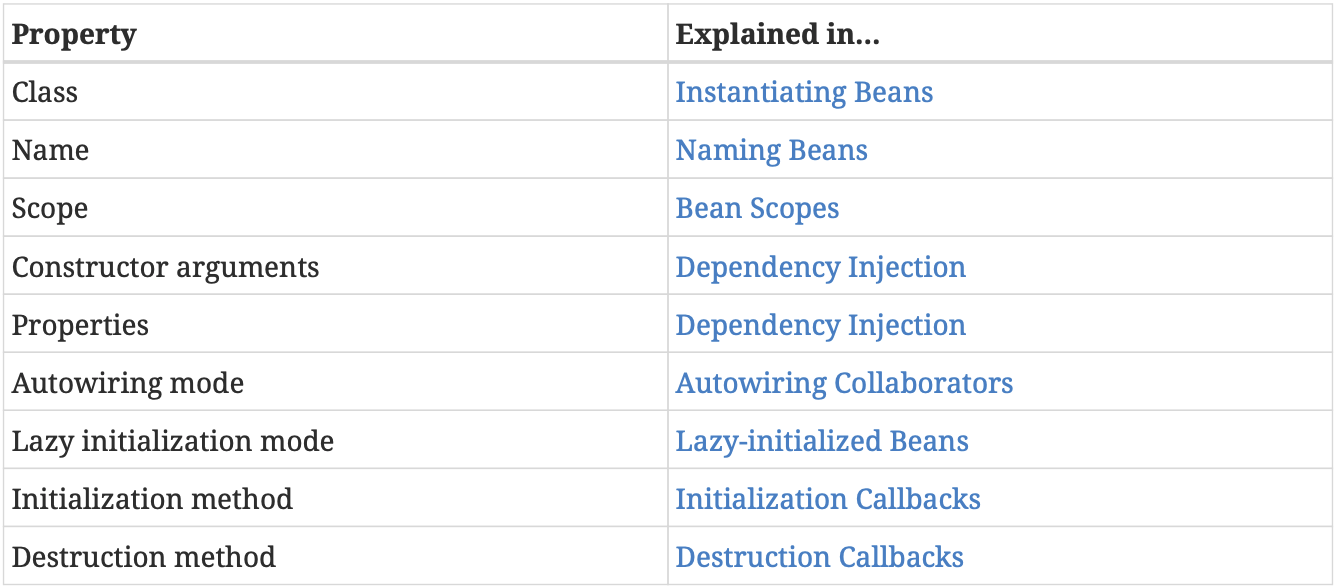
\includegraphics[width=.8\linewidth]{./Figure/IMG_bean_def.png}
%   \end{figure}

除了包含有关如何创建特定bean的信息的bean定义之外,
ApplicationContext实现还允许注册在容器外部(由用户)创建的现有对象。
 这是通过通过getBeanFactory()方法访问ApplicationContext的BeanFactory来完成的
 ,该方法返回BeanFactory DefaultListableBeanFactory实现。
  DefaultListableBeanFactory通过registerSingleton(..)和registerBeanDefinition(..)
  方法支持此注册。 但是,典型的应用程序只能与通过常规bean定义元数据定义的bean一起使用。

\chapter{Spring中的面向切面编程}
面向切面编程是面向对象编程的补充,它提出了另一种对程序结构的思考方式。
在OOP中,最重要的模块是类,而在AOP中,最重要的模块是\textit{切面}。
切面使程序的关注点模块化,例如可以通过AOP实现跨多种类型和对象的事务管理
(这类关注点在关于AOP的文献中通常被称为横切关注点)。

AOP 框架是Spring中最重要的组件之一。
AOP组件并不和Spring的IoC 容器强绑定,你可以在不引入AOP的情况下使用容器。
AOP为 Sping的IoC提供一种非常强大的中间件解决方案。

在Spring框架中,AOP常被用于:

\begin{itemize}
    \item 提供声明式的企业服务,最重要的此类服务是声明式事务。
    \item 允许开发者实现自定义的切面来使用AOP扩展OOP。
\end{itemize}

\section{AOP中的概念}
首先介绍一下在AOP中的一些主要概念和术语。
这些概念和术语并不是Spring定义的,不过它们含义并不是很特别直观。
如果由Spring使用自己的概念和术语,可能反而会令开发者更加困惑。

\begin{itemize}
    \item 切面:可以涉及不同类的模块化关注点。 事物管理是
    企业Java应用程序中横切关注点的一个很好的例子。 在Spring AOP中,切面
    使用常规类(基于配置声明的方式)或@Aspect带注释的常规类实现
    (基于@AspectJ的方式)。
    \item 连接点:程序执行过程中的某一时刻,例如方法执行或异常处理。
     在Spring AOP中,连接点始终是方法执行。
    \item 增强:切面在某个连接点执行的操作,有前置、后置、环绕等增强方式(下文介绍)。
    在包括Spring在内的众多AOP框架中,
    都会将增强实现为一个拦截器,然后将多个拦截器组装成一个作用于连接点的拦截器链。
    \item 切点:是一个谓词表达式,用来计算是否匹配连接点。
    增强与切点表达式相关联
    并切会在匹配切点表达式的连接点上执行(例如,指定匹配特定名称的方法)。
    被切入点表达式匹配的连接点是AOP的核心概念。
    默认情况下,Spring使用AspectJ切点表达语言。
    \item 引入:在个对象中声明额外的方法或字段。
    Spring AOP允许开发者向被增强的对象引入新的接口以及对应的实现。
    例如,开发者可以使用引入来使Bean实现IsModified接口,以简化缓存。
    (在AspectJ社区中,引入也被称为跨类型声明)
    \item 目标对象:被一个或多个切面增强的对象,即“被增强对象”。
    由于Spring AOP是使用运行时代理实现的,因此对象始终是被代理对象。
    \item AOP 代理:AOP框架为了实现切面(增强方法执行等)而创建的对象。在Spring框架中,一个AOP 代理对象要么是JDK动态代理创建的,要么是GCLIB创建的。
    \item 织入:将切面与其他类型或对象链接以创建一个被增强对象的过程。织入可以在编译时(使用AspectJ 编译器)、加载时和运行时执行。
    像其他纯Java实现的AOP框架一样,Spring AOP 在运行时完成织入。
\end{itemize}

增强的种类:

\begin{itemize}
    \item 前置增强:在连接点之前执行增强,但是并不能阻碍连接点之后的程序执行,除非在增加执行的过程中抛出异常。
    \item 返回后增强:在连接点正常执行完成之后执行增强,比如,一个方法正常执行完成而且没有抛出异常。
    \item 抛异常后增强:在连接点执行抛出异常之后执行增强。
    \item 后置增强:不论连接点是否正常执行完成,都会在之后执行增强。
    \item 环绕增强:环绕连接点(例如方法执行)执行的增强,是最强大的增强类型。
    环绕增强可以在方法执行之前和执行完成之后执行定制化的逻辑。因此它还能控制是否继续执行连接点之后的代码,
    可以选择抛出异常、返回连接点的执行结果或者返回增强自己的结果。
\end{itemize}

环绕增强建议是最通用的增强。
Spring AOP与AspectJ一样,提供了各种增强类型,
因此我们建议开发者使用功能最弱的建议类型来实现所需的额外操作。
例如,如果只需要用方法的返回值来更新缓存,
则最好使用返回后增强而不是环绕增强,尽管环绕增强可以完成相同的事情。
使用最合适的增强类型可以使编程模型更简单,并减少出错的可能性。
例如,开发者不需要在环绕增强的JoinPoint上调用proceeed()方法,所以也不会导致调用失败。

所有增强的参数都是静态类型的,
因此开发者可以使用参数的确切类型(例如,方法返回的值的类型)而不是对象数组类型。

匹配切点的连接点是AOP的关键概念,它与仅提供拦截功能的旧技术有所不同。
切点使增强独立于面向对象的层次结构中。
例如,开发者可以将提供声明性事务管理的环绕增强应用于多个对象(例如服务层中的所有业务操作)的一组方法。

\section{Spring AOP能力和目标}
Spring AOP是用纯Java实现的。 不需要特殊的编译过程。 
Spring AOP不需要控制类加载器的层次结构,因此适合在Servlet容器或应用程序服务器中使用。

Spring AOP当前仅支持方法执行连接点(增强在Spring Bean上执行方法)。
尽管可以在不破坏核心Spring AOP API的基础上添加对字段侦听的支持,但是目前暂未实现。
如果需要增强字段的访问和更新的连接点,可以考虑使用诸如AspectJ之类的语言。

Spring AOP的实现方法不同于大多数其他AOP框架。 
其目的不是提供最完整的AOP实现(尽管Spring AOP相当强大),
而是在AOP实现和Spring IoC之间提供紧密的集成,以帮助解决企业应用程序中的常见问题。

因此,通常将Spring 框架的AOP功能与IoC容器结合使用。
通过使用常规bean定义语法来配置切面(强大的“自动代理”功能)。
这是与其他AOP实现的关键区别。
使用Spring AOP有时候无法轻松或高效地完成某些事情,例如增强非常细粒度的对象(通常是域对象)。
在这种情况下,AspectJ是最佳选择。
但是,大部分情况下,Spring AOP为
AOP可以解决的企业Java应用程序中的大多数问题
提供了出色的解决方案。

Spring AOP从未在提供全面的AOP解决方案上与AspectJ竞争。
 我们认为,基于代理的框架(例如Spring AOP)和成熟的框架(例如AspectJ)都是有价值的,
 并且它们是互补的,而不是竞争。 
 Spring无缝地将Spring AOP和IoC与AspectJ集成在一起,
 使得在基于Spring的一致应用程序架构中支持AOP的所有使用。
  这种集成不会影响Spring AOP API或AOP Alliance API。
   Spring AOP保持向后兼容。 有关Spring AOP API的讨论,请参见下一章。

\section{AOP代理}
Spring AOP默认使用标准JDK动态代理实现AOP代理,因此可以代理任何接口(或一组接口)。

Spring AOP也可以使用CGLIB代理。 
在需要对类进行代理的情况下,基于CGLIB的代理是必须的。 
默认情况下,如果业务对象未实现接口,则使用CGLIB。 
面向接口编程是行业规范,因此业务类通常实现一个或多个业务接口。 
当需要增强未在接口上声明的方法或需要将代理对象作为具体类型传递给方法的情况下(在极少数情况下),
可以强制使用CGLIB。

掌握Spring AOP是基于代理实现的这一事实是非常重要。 
要了解具体实现细节,请参阅了解AOP代理。